\chapter{Fundamentação Teórica}

Matemática financeira é um ramo da Matemática que se utiliza de uma série de conceitos matemáticos para realizar a análise de dados financeiros em geral. Para a implementação da \textit{PyFinancial} foram considerados os principais conceitos financeiros existentes na HP-12C, conforme presente no Apêndice \ref{glossario}.

É importante ressaltar que durante a pesquisa realizada no intuito de coletar as fórmulas financeiras relacionadas aos conceitos implementados, percebeu-se que várias são as fórmulas existentes e divulgadas na Internet, porém muitas delas não apresentam resultados similares aos da HP-12C. Com isso, à medida que são apresentados os conceitos é interessante observar as fórmulas que estão implementadas e que se encontram no Apêndice \ref{formulas}.

Abaixo tem-se uma breve explicação dos principais conceitos financeiros utilizados na \textit{PyFinancial}.

\section{Conceitos}

\subsection{Considerações iniciais}

Aplicações financeiras partem de um capital inicial e este é aplicado a uma certa taxa de juros, podendo ser esta aplicação configurada por uma série simples ou complexa, de modo a gerar, com o passar do tempo, um capital final que implique em alguma remuneração ou perda. Esses juros são aplicados ao capital de acordo com a capitalização fixada para o investimento. Como exemplos temos investimentos em poupança, empréstimos, etc.

Uma forma simples de ter-se uma idéia de como funciona uma dessas movimentações é observando o fluxo de caixa da mesma através de um diagrama de tempo. Um exemplo desse diagrama pode ser visto na Figura \ref{fluxo}. Nele temos representado uma entrada no tempo inicial e a realização de dois pagamentos em dois instantes distintos de tempo.

\begin{figure}[!h]
 \centering
 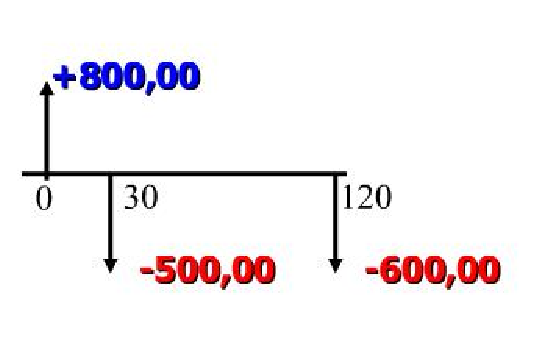
\includegraphics[scale=0.8]{fluxo.eps}
 \caption{\it Diagrama de Fluxos de Caixa.} \label{fluxo}
\end{figure}

\subsection{Valor Presente (VP)}

Aplicações têm início com uma quantia a partir de um marco inicial. Essa quantia corres\-ponde à quanto vale o investimento inicialmente, sem análises do futuro. A esse valor, que pode ser um valor gasto ou recebido, dá-se o nome de Valor Presente ou valor atual. Um exemplo seria uma pessoa que aplica R\$ $500,00$ na poupança. Esse valor seria o valor presente de sua aplicação. Assim, valor presente, capital inicial e valor atual têm o mesmo significado.

O valor presente de uma dada prestação pode ser entendido como sendo o valor no ins\-tante zero de uma certa prestação futura descontada dos juros.

\subsection{Valor Presente Líquido (VPL)}

Uma vez que o valor presente está definido, bem como as prestações, juros da movimentação e número de períodos durante os quais a aplicação estará vigente, uma análise bastante comum é verificar qual o valor da aplicação atualmente. Ou seja, para cada prestação descontam-se os juros existentes, sejam estes simples ou compostos, considerando a quantidade de períodos até que a prestação fosse paga e obtém-se o valor da prestação na data-pólo inicial. Em seguida somam-se os valores presentes de cada prestação ao valor presente e obtém-se o VPL.

Um VPL positivo é um indicativo de que a aplicação possui um retorno positivo para o aplicante e que pode ser considerada. Já um VPL negativo indica que a aplicação não deve ser considerada. \cite{vpl}

Uma consideração importante a ser realizada é que esse valor presente líquido pode ser calculado de duas formas diferentes: uma com pagamentos postecipados e outra com pagamentos antecipados.

\subsection{Valor Futuro (VF)}

Considerando o valor presente, os juros, as prestações e um dado período de vigência, o valor futuro de uma dada aplicação é o valor obtido ao final da mesma. Ou seja, o valor futuro é o resultado da incidência dos juros e das prestações sobre o valor presente. Esse valor também é conhecido como capital final.

É importante destacar que, da mesma forma que o VPL, o valor futuro é influenciado pelo fato de estar-se trabalhando com pagamentos antecipados ou postecipados. Logo, dependendo do tipo de pagamento em vigência têm-se diferentes valores futuros.

\subsection{Taxa de juros (I) e Taxa interna de retorno (TIR)}

Os juros, ou taxa de juros, de uma dada aplicação é o percentual que será aplicado sobre um montante de modo a gerar a remuneração da aplicação. Essa remuneração pode ser feita através de um sistema de juros compostos ou ainda de um sistema de juros simples.

A taxa interna de retorno, por sua vez, é a taxa de juros que iguala o valor presente das entradas ao longo da aplicação ao valor presente das saídas da aplicação. Ou seja, podemos entendê-la como o valor da taxa de juros que torna o valor presente líquido do investimento igual a zero, a aplicação não fez diferença.

Se a taxa de juros considerada para a aplicação for menor que a TIR então é um indicativo de que a aplicação é atrativa, se for maior a aplicação não deve ser considerada e sendo igual implica que a aplicação não fará diferença\cite{irr}. 

Por exemplo, suponha que uma empresa invista R\$ 30.000.000,00 para obter fluxos futuros de R\$ 11.000.000,00, R\$ 12.100.000,00 e R\$ 13.310.000 ao longo de três anos. A taxa interna de retorno do investimento é de 10\% ao ano. Assim, se a taxa de juros do mercado fosse de 6\% teria-se um VPL de R\$ 2.321.648,00, ao passo que se a taxa de juros fosse 15\% teria-se um VPL de R\$-2.533.903,00. Portanto, conclui-se que quanto maior for a TIR, maior será o número de possibilidades do investimento ser lucrativo. 

\subsection{Número de Períodos (n)}

O número de períodos indica quantas vezes a taxa de juros será aplicada em uma certa aplicação de modo a gerar remuneração. Além disso, o número de períodos também informa os locais no tempo onde pode haver entradas ou saídas no fluxo.

\subsection{Prestações (pmt)}

As prestações indicam entradas ou saídas de capital em um certo fluxo de caixa. Tipicamente nos cálculos considera-se uma prestação negativa para representar uma saída de capital e uma prestação positiva para representar uma entrada. Por exemplo, pode-se pensar em uma empresa que recebe um montante de R\$ $60.000,00$ a cada ano e gasta um total de R\$ $20.000,00$, tem-se que o \textit{pmt} a ser considerado para a aplicação da mesma é R\$ $40.000,00$.


\subsection{Sistema de amortização (SA)}

Um sistema de amortização indica como um determinado financiamento é pago ao longo do tempo. Para isso, definem-se o valor das prestações que inclui tanto o montante a ser abatido do saldo devedor, bem como os juros a serem pagos. Assim, pode-se entender como amortização a diminuição do saldo devedor, ou dívida, que pode ser realizada em etapas ou de uma única vez.

Dentre os sistemas de amortização mais famosos é comum citar o Sistema de Amortização Francês (SAF), ou \textit{Tabela Price}, e o Sistema de Amortização Constante (SAC). Atualmente o SAC é bastante utilizado no Sistema de Financiamento Habitacional, em especial pela Caixa Econômica Federal, e o SAF é amplamente utilizado pelos bancos em seus sistemas de Crédito Direto ao Consumidor (CDC), bem como nas vendas a prazo divulgadas pelas grandes redes de varejo \cite{usoSACSAF}.

